%----------------------------------------------------------------------
% Problem 1

\begingroup
\allowdisplaybreaks

\newpage
\section{Problem 1}

\textbf{Exercise 2 in Section 3.6}

\subsection{Solution}
	
\textbf{Note: } \textit{My MATLAB code for this homework problem repeats all the steps for example 3.1 so that I can take on this problem. I will only cover the checkerboard test in this write-up.}
\newline

The checkerboard test using $\bv{m}_{true}$ can be reshaped to $\bv{m}_{true} \in \R^9$ such that

\begin{align*}
	\bv{m}_{true} = \begin{bmatrix}
		-1 & 1 & -1 & 1 & -1 & 1 & -1 & 1 & -1
	\end{bmatrix}^T
\end{align*}

which allows for the creation of test data $\bv{d}_{true}$ and a recovered model $\bv{m}_{\dagger}$.

\begin{align*}
	\bv{d}_{true} &= G \bv{m}_true \\
	\\
	\bv{m}_{\dagger} &= G^{\dagger} \bv{d}_{true}
\end{align*}

Recall from example 3.1 that $G \in \R^{8 \times 9}$ with rank $7$. Therefore the generalized pseudo-inverse of $G$, represented as $G^{\dagger}$, was computed using the Moore-Penrose pseudo-inverse function \verb*|pinv(G)| in \MATLAB. Figure \ref{fig: prob1 checkerboard test} shows how the recovered model compares to the true model. 

\begin{figure}[h] 
	\centering
	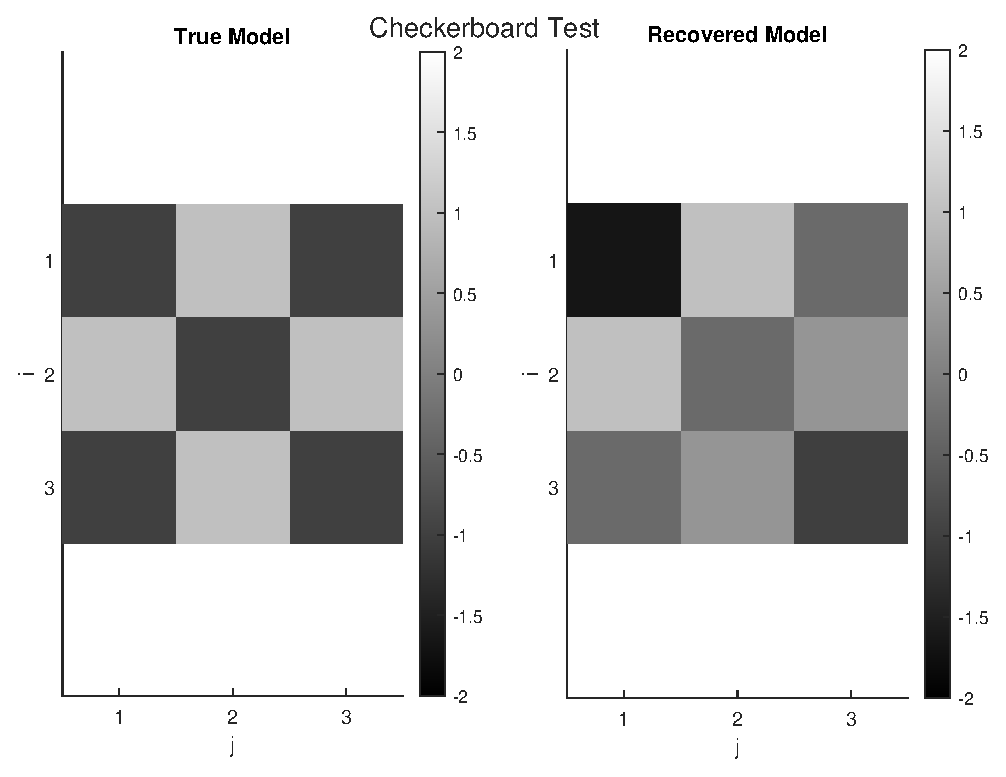
\includegraphics[width=0.85\textwidth]{./images/prob1_checkerboard_test.eps}
	\caption{Checkerboard Test}
	\label{fig: prob1 checkerboard test}
\end{figure}
\FloatBarrier

Interpreting these results, only three of nine model parameters $m_2, m_4, m_9$ were recovered with no error. The error in the recovered model, $\Delta \bv{m} \defeq \bv{m}_{\dagger} - \bv{m}_{true}$, is shown below.

\begin{align*}
	\Delta \bv{m} = \begin{bmatrix}
		\frac{-2}{3} & 0 & \frac{2}{3} & 0 & \frac{2}{3} & \frac{-2}{3} & \frac{2}{3} & \frac{-2}{3} & 0
	\end{bmatrix}^T
\end{align*}

